%
% 合同ゼミ資料 サンプル (2023年upLaTeX版)
%
\documentclass[autodetect-engine,dvi=dvipdfmx,ja=standard,plautopatch=true,
               a4,twoside,10pt]{bxjsarticle}
\usepackage{godozemi2023}

%-----------------
%     Preamble
%-----------------
\usepackage{graphicx}
\usepackage[font=footnotesize]{subfig}

\usepackage{enumerate}
\usepackage{url}

\usepackage{amsmath}
\usepackage{amssymb}

% 草稿用
%\IsDraft % ヘッダにコンパイルした日付時刻を挿入
%\usepackage{showkeys} % ラベルを表示する

%% 行間を調整するパラメータ。規定ページ内に収めるときの最終手段。
\def\baselinestretch{0.95}


%-----------------
%       body      
%-----------------

\begin{document}
%---------------------------------------
% タイトル部
\jeheader %
%% 表題(和・英)
  {聴取者の主観評価に基づく音地図作成のための環境音収録}
  {Sound recording to construct sound-map on the basis of listener's subjective evaluation}
%% 著者(和・英)
  {原 直}
  {Sunao Hara}
%% 所属(和・英)
  {岡山大学 阿部研究室}
  {Abe Laboratory, Okayama University}
%---------------------------------------

%---------------------------------------
% 概要(目安は200文字程度)
\abstract{%
本研究では,「聴取者の主観を含んだ音の収集」と「大規模な音の物理量の収集」という
二つのデータ収集を通して,聴取者の主観を伴った大規模な環境音データベース構築を目指す.
Participatory sensingとOpportunistic sensingというクラウドセンシングの考え方に着目する.
本報告では長時間にわたる特定地域での環境音収録を行い,
収録された騒音レベルの可視化において聴取者の主観を反映させる方式について検討を行った.
} % end-of-abstract
%---------------------------------------


%====================
\section{はじめに}
環境音は人が環境を理解するための重要な情報の一つであるが,
聴取者の状況や主観的な印象によって環境音の印象が変化することがある.
例えば音の大きさの物理量として騒音レベルが知られているが,
同じ騒音レベルの環境音でも場の状況や聴取者により主観的な音の大きさは異なると考えられる.
従って環境音の研究を進めるためには聴取者の主観を伴った大規模な環境音データベースが必要である.

大量のデータを集めるには
ライフログ\cite{Mesaros_EUSIPCO2010,Shah_ESPA2012}や
クラウドソーシング\cite{Rana2010_IPSN_EarPhone,DHondt2012_Journal_NoiseTube}の
アプローチが有効である.
しかし,ライフログとしての環境音の収集は聴取者の主観を含んだデータが収集できるが,
プライバシーの問題から研究用データベースへの活用は容易ではない.
一方で,クラウドソーシングのアプローチに基づく環境音収集においてプライバシーに配慮するならば,
音そのものではなく音の特徴の一部を表した物理量を収集することは可能と考えられる.

本研究では,
「聴取者の主観を含んだ音の収集」と「大規模な音の物理量の収集」という
二つのデータ収集を通して,聴取者の主観を伴った大規模な環境音データベース構築を目指す.
これまでにスマートデバイスによる環境音収録アプリケーションの開発と
収録実験を行ってきた\cite{Hara2014_ASJ1409}.
本報告では長時間にわたる特定地域での環境音収録を行い,
収録された騒音レベルの可視化において聴取者の主観を反映させる方式について検討を行った.

%====================
\section{環境音収録アプリケーション}

本研究で実施する収録実験のために,
環境音収録アプリケーション\cite{Hara2014_ASJ1409}を改良した.
このアプリケーションでは,音を保存する際に,
その場の音を主観的に評価するために騒音度と混雑度の5段階評価を与える事ができる.
さらに,その場の状況や聞こえてくる音を記録するために,
任意のテキスト入力エリアと12種類のあらかじめ設定された音の種類が用意されている.
ユーザはツイートボタンを押すことで様々な情報を付与した音声を記録することができる.
システムは,ツイートボタンが押されると,
リングバッファから直近10秒の音声波形をRIFF wavファイルとして作成すると同時に,
主観評価の選択項目とテキスト入力の内容を表す文字列に時間をつけてログファイルに記録する.
アプリケーションでは「音声」,「位置履歴ログ」,
「騒音レベルログ」,「ツイートログ」がそれぞれファイルとして生成される.

音声は量子化ビット数16~bit,サンプリングレート32000~Hzで収録が行われる.
1秒毎に得られる音声サンプル $x[n], n=1,\dots,N$に対してA特性$A[k]$に基づく等価騒音レベル$L_{eq}$ を以下の計算式で計算する.
\begin{align}
    X[k] &= \frac{1}{N} \sum_{n=0}^{N-1} x[n] \cdot e^{-2 \pi j k n/N} \\[-3pt]
	L_0 &= 10 \log_{10} \frac{1}{K} \sum_{k=0}^{K-1} \Bigl| A[k] \cdot X[k] \Bigr|^2 \\[-3pt]
	L_{eq} &= B(L_0)
\end{align}
ここで,$N$は計算に用いる信号長であり,$K$はFFT長($K>N$)であり,
$B(\cdot)$は量子化された音声波形のパワーを音圧レベル値に変換する関数である.
本報告では1秒間に相当する$N=32000$を利用し,
$B(\cdot)$は騒音計(RION NL-42)を用いて事前に収録された校正値の線形補間により関数を作成した.


%====================
\section{環境音収録}

%--------------------
\subsection{収録の概要}

6名の実験参加者によって岡山市内の4地域を重点的に収録した.
4地域の主な属性は「閑静な住宅地」,「駅前」,「駅に近い商店街」,「駅からやや離れた商店街」である.
収録は2014年11月22日から29日の間で,平日2日と土日2日の合計4日間として,
1日あたり2地点を3名ずつ巡回することで午前8時から午後9時までの環境音と等価騒音レベルを収録した.
1時間を1セッションとして地域毎に定めた経路を巡回する.
巡回時には端末(Google Nexus~7)を手に持ったまま収録しており,
経路上の特定の位置で主観評価や環境音の収録を行うように指示した.

主観的な騒音度合いの選択肢は,
$L_1$: とても静か,
$L_2$: 比較的静か,
$L_3$: やや騒がしい,
$L_4$: かなり騒々しい,
$L_5$: とても騒々しい,
の5段階である.
また,主観的な混雑度合いの選択肢は,
$C_1$: 誰もいない,
$C_2$: まばら,
$C_3$: やや多い,
$C_4$: かなり多い,
$C_5$: 混雑,
の5段階である.
環境音の種類は\tabref{tbl:SoundTypeHistogram}の12種類として,複数選択を可能にした.
参加者には,すべての項目を埋める必要はないことを指示している.

%--------------------
\subsection{収録データの予備分析}

収録実験により収集された位置履歴ログファイルと騒音ログファイルの時間同期を行った結果,
緯度経度と等価騒音レベルをすべて持つデータは367,242組得られた.
音声データの総数は2,740サンプルであり,全て10秒の音声ファイルである.
収録された音声データにつけられた環境音ラベル毎の頻度分布を
\tabref{tbl:SoundTypeHistogram}に示す.

%------------------- TABLE  START -------------------%
\begin{table}[tb]
\centering
	\caption{収録された環境音の出現頻度分布}
	\label{tbl:SoundTypeHistogram}
\resizebox{\columnwidth}{!}{%
	\begin{tabular}{llr|llr}
	\Hline
	\multicolumn{2}{l}{Class} & \#data & \multicolumn{2}{l}{Class} & \#data \\
	\hline
	$T_1$ &	人の声      & 1356 & $T_{7}$  & 踏切の音   &   1 \\
	$T_2$ &	鳥の声      &  634 & $T_{8}$  & 電車の音   &  97 \\
	$T_3$ &	虫の音      &   56 & $T_{9}$  & サイレン音 &  37 \\
	$T_4$ &	車の音      & 2267 & $T_{10}$ & 音響信号機 & 788 \\
	$T_5$ &	風切音      &  185 & $T_{11}$ & 音楽     &   374 \\
	$T_6$ & バイクの音  &  727 & $T_{12}$ & 動物の声 &    61 \\
	\Hline
	\end{tabular}
} % resizebox
\end{table}
%-------------------  TABLE  END  -------------------%

等価騒音レベルの可視化を行った例を\figref{fig:soundmap_loudness_screenshot}に示す.
この図は収録実験で得られたデータから緯度経度を座標軸とした二次元ヒストグラムによる集計を行い,
平均値をその地域の代表的な騒音レベルとして色分け表示している.
可視化システムではアニメーション表示をしており,時間帯の移り変わりに伴う音の変化を見ることが観察できる.

%------------------- FIGURE START -------------------%
\begin{figure}[tb]
\centering
	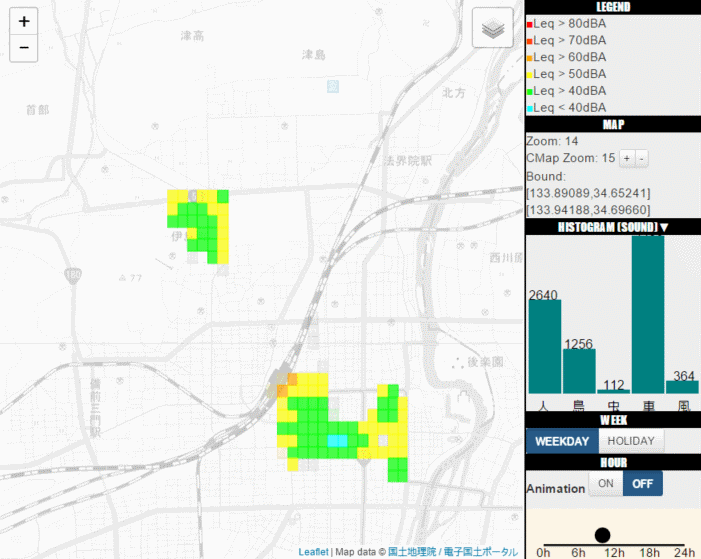
\includegraphics[width=.75\columnwidth]{img/soundmap_screenshot_rev150121_s.png}
	\caption{地図上での環境音可視化システム(騒音表示)}
	\label{fig:soundmap_loudness_screenshot}
\end{figure}
%-------------------  FIGURE END  -------------------%


\subsection{等価騒音レベルと主観評価の比較}

\figref{fig:Loudness}は主観評価に対する等価騒音レベルの平均値を示している.
収録データ数が少ないことから,「かなり多い($C_4$)」と「混雑($C_5$)」は一つのクラス$C_{4,5}$とした.
いずれの図についても主観的な感覚と客観的な指標がおよそ一致していることから,
人による評価のばらつきは小さいと考えられる.
ただし,\figref{fig:Loudness_SubjLoudness}において「とても騒々しい($L_5$)」の信頼区間が広がっていることから,
「かなり騒々しい($L_4$)」との弁別基準は人によるばらつきが大きいことが示唆される.

%------------------- FIGURE START -------------------%
\begin{figure}[t]
	\centering
	\subfloat[Subjective loudness]{ %
		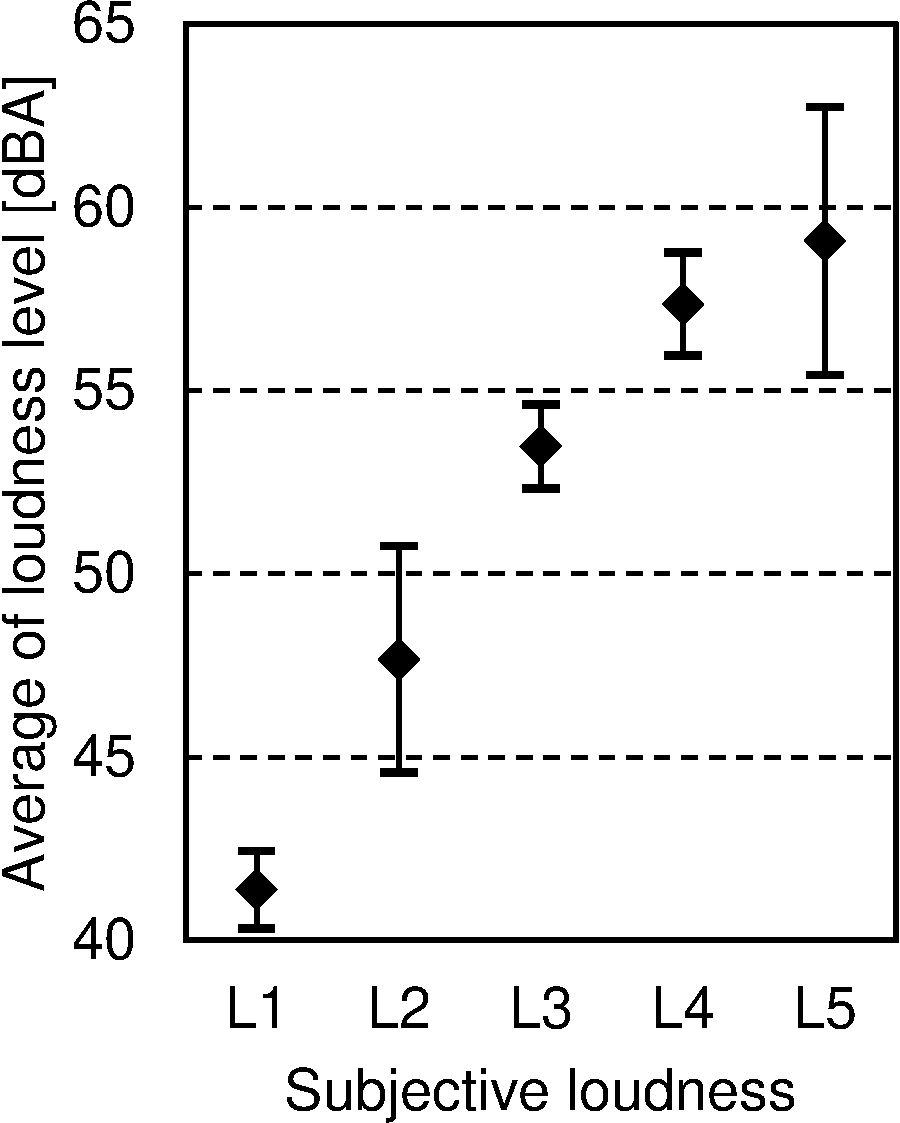
\includegraphics[width=.425\columnwidth]{img/Loudness_SubjL_Boxplot-crop.pdf} %
		\label{fig:Loudness_SubjLoudness}
	} %
	\hspace{0.05\columnwidth}
	\subfloat[Subjective crowdedness]{ %
		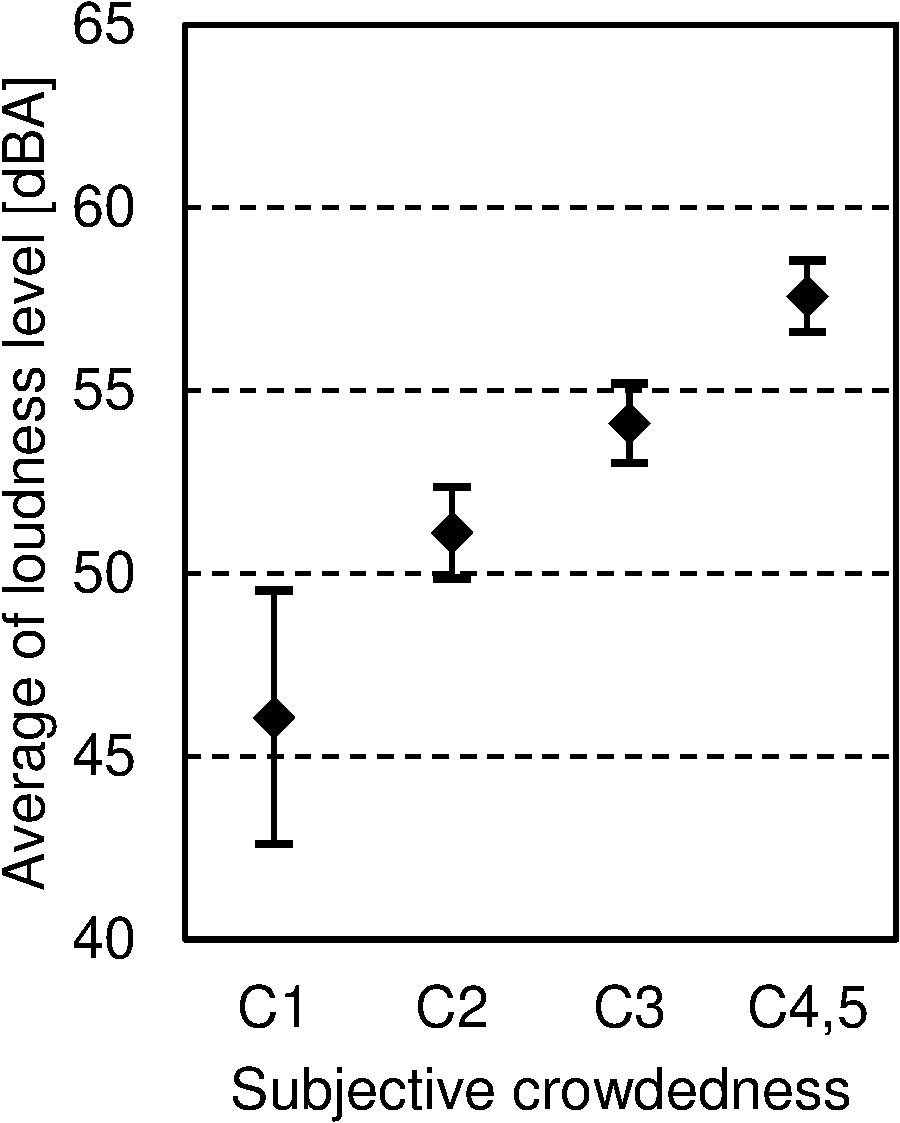
\includegraphics[width=.425\columnwidth]{img/Loudness_SubjC_Boxplot-crop.pdf} %
		\label{fig:Loudness_SubjCrowdedness}
	} %
	\caption{主観評価に対する等価騒音レベルの平均値.エラーバーは90\%信頼区間を示す.}
	\label{fig:Loudness}
\end{figure}
%-------------------  FIGURE END  -------------------%


%====================
\section{まとめ}

本報告では,タブレット型端末を用いた岡山市4地域における環境音収録について述べた.
また,主観的な混雑度合いの可視化に向けたGMM-UBMによる推定手法について検討した.
推定の有効性は示唆されたが,今後は推定手法の詳細な検討が必要である.


%-----------------
%   Bibliography      
%-----------------
%% You can use (1) bibtex,
%\bibliographystyle{ieicex}  % Bib-style
%\bibliography{mybib}        % Bib-database
%% , or (2) write them directory in this document.
\begin{thebibliography}{9}
 \setlength\itemsep{4pt}    % アイテム間の大きさ
 \setlength\baselineskip{11.5pt} % アイテム内の行間の大きさ

\bibitem{Mesaros_EUSIPCO2010}
  A.~Mesaros, \textit{et~al.},
  ``Acoustic event detection in real life recordings,''
  Proc. of 18th European Signal Processing Conference (EUSIPCO-2010), pp.~1267--1271, Aug. 2010.

\bibitem{Shah_ESPA2012}
  M.~Shah, \textit{et~al.},
  ``Lifelogging: Archival and retrieval of continuously recorded audio using wearable devices,''
  Proc. of IEEE International Conference on Emerging Signal Processing Applications (ESPA-2012), pp.~99--102, Jan. 2012.

\bibitem{Rana2010_IPSN_EarPhone}
  R.~Rana, \textit{et~al.},
  ``{Ear}-{Phone}: An end-to-end participatory urban noise mapping system,''
  Proc. of The 9th ACM/IEEE International Confernce an Information Proccessings in Sensor Networks (IPSN 2010), pp.~105--116, Apr. 2010.

\bibitem{DHondt2012_Journal_NoiseTube}
  E.~D'Hondt, \textit{et~al.},
  ``Participatory noise mapping works! an evaluation of participatory sensing as an alternative to standard techniques for environmental monitoring,''
  Pervasive and Mobile Computing, vol.~9, no.~5, pp.~681--694, Oct. 2013.

\bibitem{HTKBook}
  ``The {HTK} {Book},'' \url{http://htk.eng.cam.ac.uk/}.

\bibitem{Hara2014_ASJ1409}
  原他,
  ``クラウドセンシングにより収集された環境音のシンボル表現を用いた音地図構築手法,\inhibitglue''
  音講論,pp.~1535--1538,sept. 2014.

\end{thebibliography}


\end{document}
